% !TeX root = ../../main.tex
\section{Model implementation}

COMSOL was selected for detailed reactor modelling, utilising the CFD and Heat Transfer modules \cite{comsol_comsol_2020,comsol_cfd_2020,comsol_heat_2020}. A single tube of the reactor was modelled in 2D axisymmetric geometry (i.e. in cylindrical coordinates). 

\subsection{Model equations}
The physics interfaces selected in COMSOL for each domain of the reactor and their associated governing equations are described in this section.

\subsubsection{Reaction zone}

In the reaction zone of the tubular reactor, mass and heat transfer are coupled with reaction through the following equations.

\paragraph{Mass transfer: Brinkman equations}

Under the assumption of Stokes and incompressible flow, the continuity and momentum equations reduce to the following \cite{comsol_cfd_2020}
\begin{equation}
    \rho\nabla \cdot \mathbf{u}=Q_{\mathrm{m}}
\end{equation}
\begin{equation}
    \frac{\rho}{\varepsilon_{\mathrm{p}}} \frac{\partial \mathbf{u}}{\partial t} =
    -\nabla p+\nabla \cdot\left[\frac{1}{\varepsilon_{\mathrm{p}}}\left\{\mu\left(\nabla \mathbf{u}+(\nabla \mathbf{u})^{T}\right)-\frac{2}{3} \mu(\nabla \cdot \mathbf{u}) \mathbf{I}\right\}\right]-\left(\kappa^{-1} \mu+\frac{Q_{\mathrm{m}}}{\varepsilon_{\mathrm{p}}^{2}}\right) \mathbf{u}+\mathbf{F}
\end{equation}

\paragraph{Chemical reaction: Transport of concentrated species}
The transport of species $i$ is given as follows \cite{comsol_cfd_2020}
\begin{equation}
    \rho \frac{\partial}{\partial t}\left(\omega_{i}\right)+\rho(\mathbf{u} \cdot \nabla) \omega_{i}=-\nabla \cdot \mathbf{j}_{i}+R_{i}
\end{equation}
Transport due to thermal diffusion is neglected.

\paragraph{Heat transfer: Porous media}

In the porous medium, heat transfer is described by a volume-averaged combination of the solid and fluid equations, respectively \cite{comsol_heat_2020}
\begin{align}
    \rho_{\mathrm{s}} C_{p, \mathrm{~s}} \frac{\partial T_{\mathrm{s}}}{\partial t}+\nabla \cdot \mathbf{q}_{\mathrm{s}} &= \mathbf{Q}_{\mathrm{s}} \\
    \rho_{\mathrm{f}} C_{p, \mathrm{f}} \frac{\partial T_{\mathrm{f}}}{\partial t}+\rho_{\mathrm{f}} C_{p, \mathrm{f}} \mathbf{u}_{\mathrm{f}} \cdot \nabla T_{\mathrm{f}}+\nabla \cdot \mathbf{q}_{\mathrm{f}} &= \mathbf{Q}_{\mathrm{f}}
\end{align}
where local thermal equilibrium is assumed such that $T_{\mathrm{s}} = T_{\mathrm{f}} = T$.

\subsubsection{Wall}

\paragraph{Heat transfer: Solid}
\cite{comsol_heat_2020}
\begin{equation}
    \rho C_{p}\left(\frac{\partial T}{\partial t}+\mathbf{u}_{\text {trans }} \cdot \nabla T\right)+\nabla \cdot\left(\mathbf{q}+\mathbf{q}_{\mathrm{r}}\right)= \mathbf{Q}_{\mathrm{ted}}+ \mathbf{Q}
\end{equation}

\subsubsection{Coolant zone}

\paragraph{Mass transfer: $k$-$\varepsilon$ Turbulence model}
This model incorporates the turbulent kinetic energy $k$ and dissipation rate $\varepsilon$ \cite{comsol_cfd_2020}. A turbulent form of the viscosity is defined as
\begin{equation}
    \mu_{T}=\rho C_{\mu} \frac{k^{2}}{\varepsilon}
\end{equation}
whilst transport equations for $k$ and $\varepsilon$ are given by
\begin{align}
    \rho \frac{\partial k}{\partial t}+\rho \mathbf{u} \cdot \nabla k &= \nabla \cdot\left(\left(\mu+\frac{\mu_{\mathrm{T}}}{\sigma_{k}}\right) \nabla k\right)+P_{k}-\rho \varepsilon \\
    \rho \frac{\partial \varepsilon}{\partial t}+\rho \mathbf{u} \cdot \nabla \varepsilon &= \nabla \cdot\left(\left(\mu+\frac{\mu_{\mathrm{T}}}{\sigma_{\varepsilon}}\right) \nabla \varepsilon\right)+C_{\varepsilon 1} \frac{\varepsilon}{k} P_{k}-C_{\varepsilon 2} \rho \frac{\varepsilon^{2}}{k}
\end{align}
with a production term in $k$ given by
\begin{equation}
    P_{k}=\mu_{\mathrm{T}}\left(\nabla \mathbf{u}:\left(\nabla \mathbf{u}+(\nabla \mathbf{u})^{T}\right)-\frac{2}{3}(\nabla \cdot \mathbf{u})^{2}\right)-\frac{2}{3} \rho k \nabla \cdot \mathbf{u}
\end{equation}

\paragraph{Heat transfer: Fluid}
\cite{comsol_heat_2020}
\begin{equation}
    \rho C_{p}\left(\frac{\partial T}{\partial t}+\mathbf{u} \cdot \nabla T\right)+\nabla \cdot\left(\mathbf{q}+\mathbf{q}_{\mathrm{r}}\right)=\alpha_{p} T\left(\frac{\partial p}{\partial t}+\mathbf{u} \cdot \nabla p\right)+\tau: \nabla \mathbf{u}+\mathbf{Q}
\end{equation}

\subsection{Optimisation and sensitivity analysis}

\subsubsection{Secondary cooling system sizing}

\begin{figure}[h]
    \centering

    \begin{subfigure}{0.49\linewidth}
        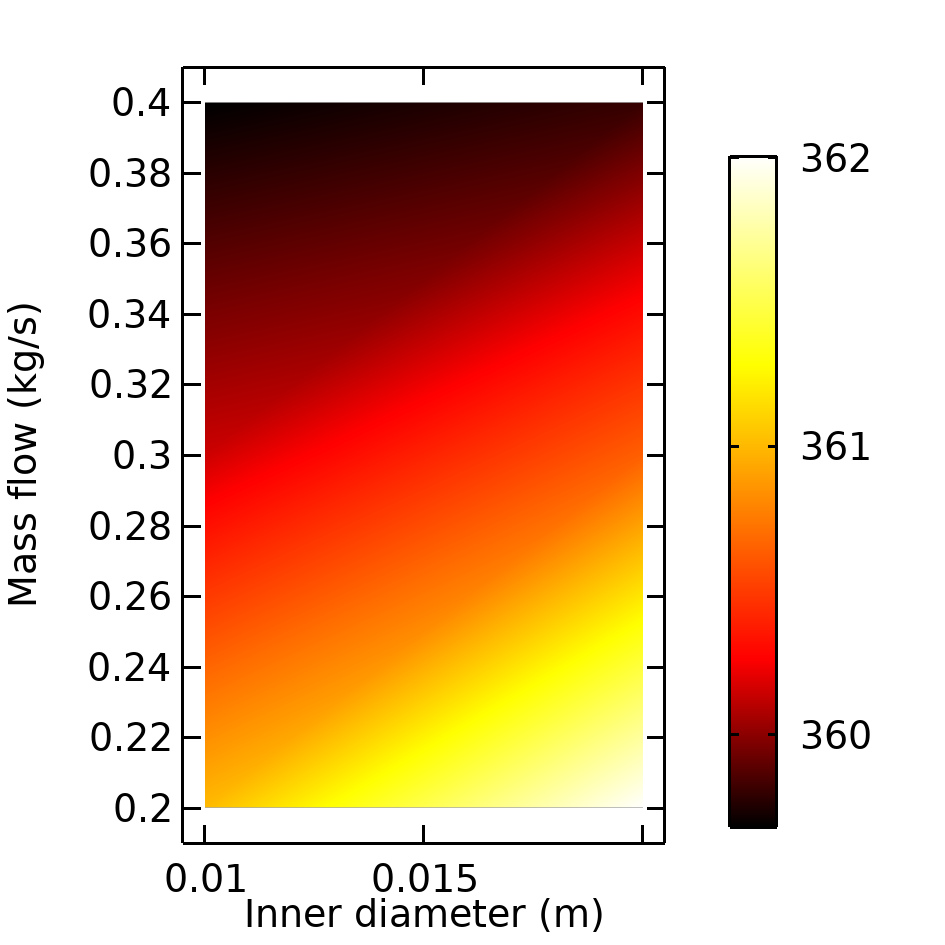
\includegraphics[width=\linewidth]{figures/S2-maxT.png}
        \caption{Maximum temperature reached in the reactor}
        \label{fig:comsol-S2:maxT}
    \end{subfigure}
    \begin{subfigure}{0.49\linewidth}
        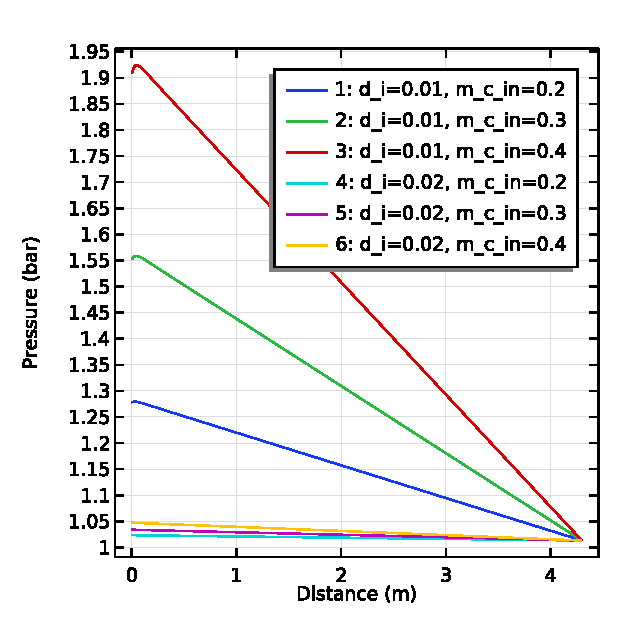
\includegraphics[width=\linewidth]{figures/S2-CW-Pdrop.eps}
        \caption{CW side pressure drop}
        \label{fig:comsol-S2:CW-Pdrop}
    \end{subfigure}

    \caption{Sensitivity to secondary CW parameters}
    \label{fig:comsol-S2}
\end{figure}
Inner coolant flowrate and diameter of inner cooling tube were optimised to keep temperature below the safe limit of 363K while maintaining a low pressure drop. As seen in Figure \ref{fig:comsol-S2:maxT}, it is desirable to have a small inner cooling tube diameter and a high coolant flowrate to keep the reactor temperature low. However, the smaller the diameter, the greater the increase in pressure drop per unit length as the coolant flowrate increases. This could be a problem in the future when the throughput is expected to increase when Nitroma's production grows. Thus, it is important to have a larger inner diameter that gives the flexibility of increasing inner coolant flowrate to remove heat from the reaction. Moreover, having a lower pressure drop means no high pressure pump is required to feed the cooling water into the reactor. The final determined values were inner diameter of 0.02m and inner coolant flowrate of 0.3 kg/s. At these specifications, the temperature of reactor can still be kept below 363K while keeping pressure drop to a minimum.

\subsubsection{Cocurrent vs counter-current cooling water flow}
[insert cocurrent vs countercurrent]
Cocurrent flow: CW warms the downstream end of the reactor, improving rate.

Countercurrent: CW removes heat from downstream section (slowing rate unnecessarily) and is then warm when it reaches the hotspot, limiting its usefulness in minimising the risk of thermal runaway.

\begin{figure}[h]
    \centering
    \begin{minipage}[t]{0.47\linewidth}
        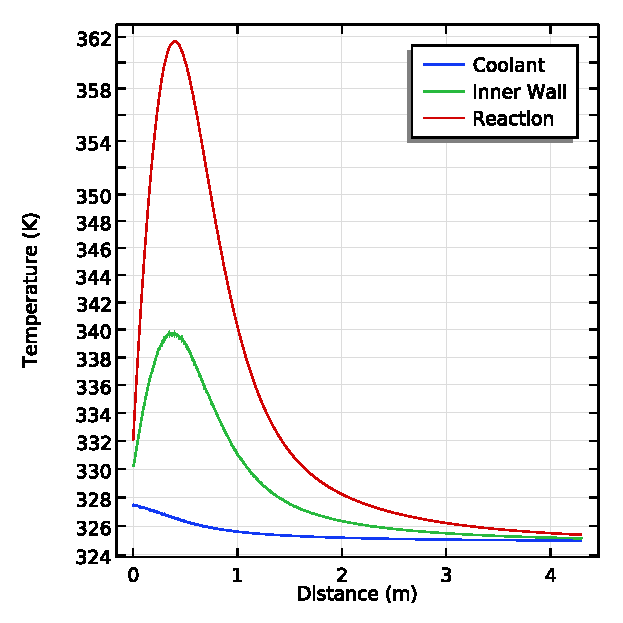
\includegraphics[width=\linewidth]{figures/temperature-lines-countercurrent.eps}
        \caption{Temperature profiles for counter-current secondary cooling water flow. Compare to \cref{fig:comsol-temperature:lines} (co-current flow).}
        \label{fig:comsol-temperature:lines:countercurrent}
    \end{minipage}\hfill
    \begin{minipage}[t]{0.47\linewidth}
        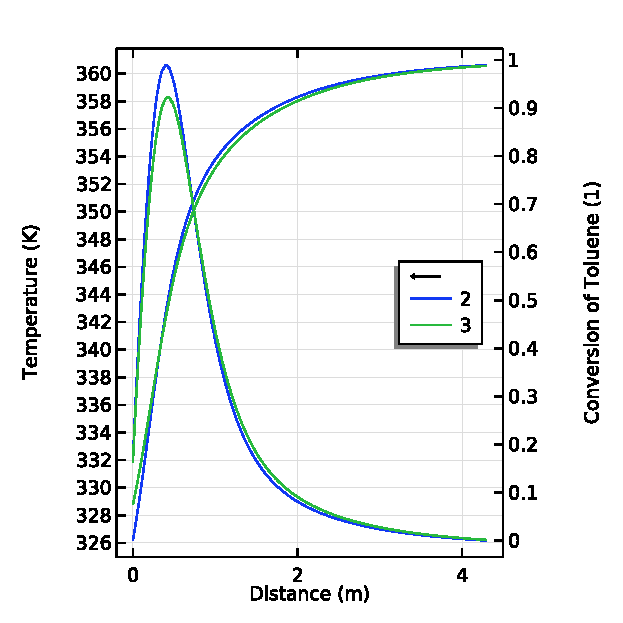
\includegraphics[width=\linewidth]{figures/S3-T-X.eps}
        \caption{Effect of changing nitric acid molar ratio on temperature and conversion profiles in reactor.}
        \label{fig:comsol-S3-T-X}
    \end{minipage}
\end{figure}

\subsubsection{\ch{HNO3} : Toluene inlet ratio}

\ch{HNO3} : Toluene molar ratio of 2 and 3 were investigated to achieve 98\% conversion in the shortest reactor length possible. Nitric acid is always kept in excess to maximise the formation of nitronium ion on the catalyst surface. Conversely, if the toluene is in excess, it will block the acid sites on the catalyst which obstructs the formation of nitronium ions [vassena et al]. 

The results showed that increasing the \ch{HNO3} : Toluene molar ratio from 2 to 3 had negligible effect on the conversion of toluene. This suggests that the surface of the catalyst had already been fully saturated. Therefore, increasing molar flowrate of nitric acid further would not enhance the conversion of the nitration reaction, but would instead lead to higher OPEX costs of supplying nitric acid to the reactor. It could also complicate the separation process of the 3 nitrotoluene isomers downstream. 

As safety is one of the key priorities of Nitroma in all decision making, the maximum temperature in the reactor were also analysed for both cases before making a final decision. Both cases were found to be below the safe temperature limit of 363K, hence, a molar flowrate ratio of 2 was selected.

\subsubsection{Number of tubes}
A sensitivity analysis was performed on the number of reactor tubes required in Figure \ref{fig:S5-T-X}. An optimal number of 7 was chosen as it provides the lowest maximum temperature at 360K and spends a comparatively short length at a maximum temperature, which will reduce the occurrence of a thermal runaway.

According to the modified Ergun equation, shown in equation \ref{eqn:ergun} the pressure drop ($\Delta p$) is inversely proportional to the length of the reactor, a shorter reactor is more favourable.  This is also evident in Figure \ref{fig:S5-T-X}, where the targeted conversion of 98\% can be achieved well within 4m of reactor length. 

The optimal number of tubes of 7 was also chosen based on the centered hexagonal number rule \cref{eqn: hexagon} which has practical usage in industry for maximising tube bundles into large cylindrical containers \cite{noauthor_realiable_2018}. 
\begin{equation}
    n^3 - (n-1)^3 = 3n(n-1)+1
    \label{eqn: hexagon}
\end{equation}
where $n$ represents the sequence of hexagonal number. The further explanation on the heat transfer benefits will be discussed in Section \ref{sec:reactortube}.


\begin{figure}[h]
    \centering
    \begin{minipage}[t]{0.45\linewidth}
        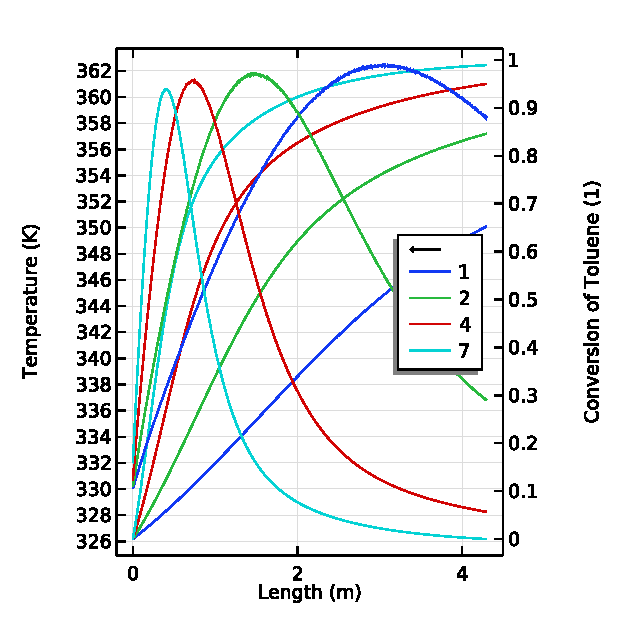
\includegraphics[width=\linewidth]{figures/S5-T-X.eps}
        \caption{Effects of changing number of tubes on reactor performance}
        \label{fig:S5-T-X}
    \end{minipage}\hfill
    \begin{minipage}[t]{0.45\linewidth}
        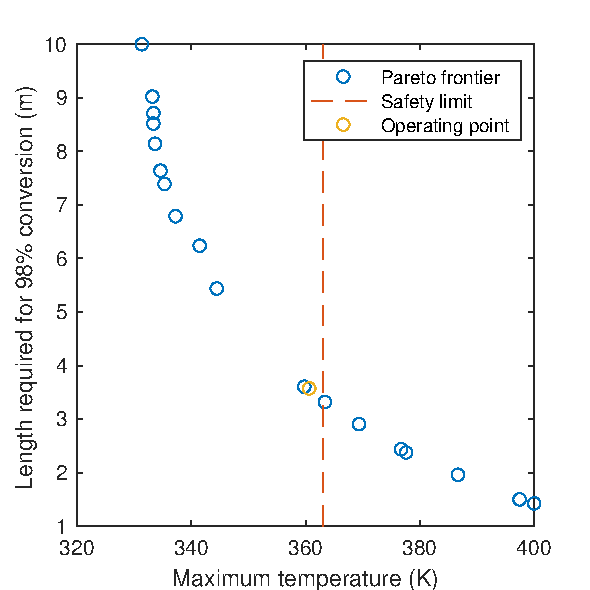
\includegraphics{figures/comsol-pareto.pdf}
        \caption{Pareto frontier for reactor performance-safety tradeoff}
        \label{fig:comsol-pareto}
    \end{minipage}
\end{figure}

\subsubsection{Pareto frontier}

A Pareto frontier illustrating the tradeoff between reactor performance (namely minimising the length required to reach the target \SI{98}{\percent} conversion) and safety (maximum temperature reached within the reactor, related to the risk of thermal runaway) was derived using the MATLAB genetic algorithm function \texttt{gamultiobj} and is shown in \cref{fig:comsol-pareto}.

\subsubsection{Coolant temperature}
\begin{wrapfigure}{R}{0pt}
    \vspace{-\intextsep}
    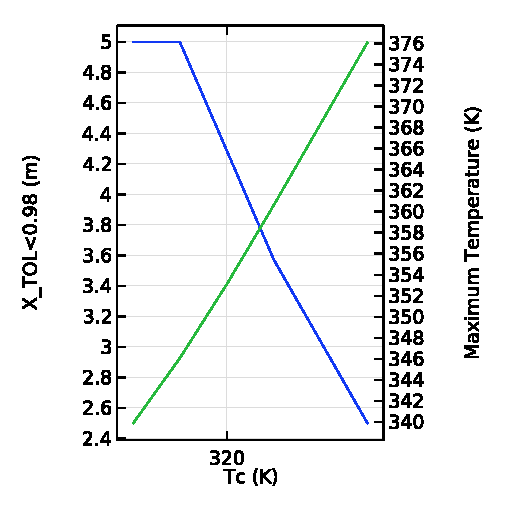
\includegraphics[width=0.5\textwidth]{figures/S4-CW-X-T.eps}
    \caption{Effect of CW temperature on distance required to reach 98\% conversion (blue) and max T (green). Maximum reactor length is capped at 5m to prevent an excessively long reactor.}
    \label{fig:comsol-S4-CW-X-T}
\end{wrapfigure}
A sensitivity analysis was performed on the cooling water inlet temperature as temperature control was deemed the most important parameter for safety and performance evaluation. The length of reactor required was found to be quite sensitive to changes in inlet cooling temperature. Any changes in temperature would have a noticeable knock-on effect on the rate of reaction since the nitration process is sensitive to temperature [chen]. The region of interest in Figure \ref{fig:comsol-S4-CW-X-T} is between \SI{325}{\K} \pm \SI{5}{\K}. Such a large fluctuation in temperature is unlikely to happen as the cooling water is sourced from a mixture of used cooling water streams across the plant and fresh cooling water. For each cooling stream to have a significant effect on the overall mixed cooling water stream temperature, there needs to be a significant deviation in the unit operations. The safety alarm systems in Nitroma's plant would alert the operators if that happens, therefore there is a low risk for the cooling water temperature to fluctuate by \pm \SI{5}{\K}. However, a conservative approach is taken when designing the HEX reactor. In the ideal scenario where the cooling water temperature does not fluctuate, a conversion of 98\% can be achieved in 3.6m as shown in Figure \ref{fig:comsol-conversion}. When taking into account the maximum deviation of \pm \SI{5}{\K}, the reactor length is extended and the final reactor length is determined to be \SI{4.2}{\metre}. The summary of cooling water stream used in the HEX reactor can be found in Appendix \ref{tab:cwtable}.

\subsection{Final results}
\label{finalresults}
Using the optimised parameter values above, the reaction was simulated in the nitration reactor. It showed robust performance by meeting the desired safety and reaction performance benchmark.

The reactor sees a sharp rise in conversion (\approx 80\%) in the first 1m of reactor before achieving the remaining 20\% in the next \approx 3m. This can be explained by the rate of reaction as shown in Figure \ref{fig:comsol-performance:r_TOL}. As high concentrations of reactants are first mixed together at the inlet of the reactor, the reaction proceeds at the highest rate in the first 0.5m before gradually decreasing after that. This results in a spike in temperature (Figure \ref{fig:comsol-temperature}) since the reaction is an exothermic process, but the combined effect of lower remaining concentration of reactants and the cooling water keeps the temperature below the safe temperature limit of 363K. A 98\% conversion that is desired for the nitration reaction was achieved within the reactor. As expected, the more valuable ONT and PNT were produced in much greater amounts as compared to MNT. These products are later fed to other parts of Nitroma's plants to be converted to final products to be sold.

\begin{figure}[h]
    \centering

    \begin{subfigure}{0.45\linewidth}
        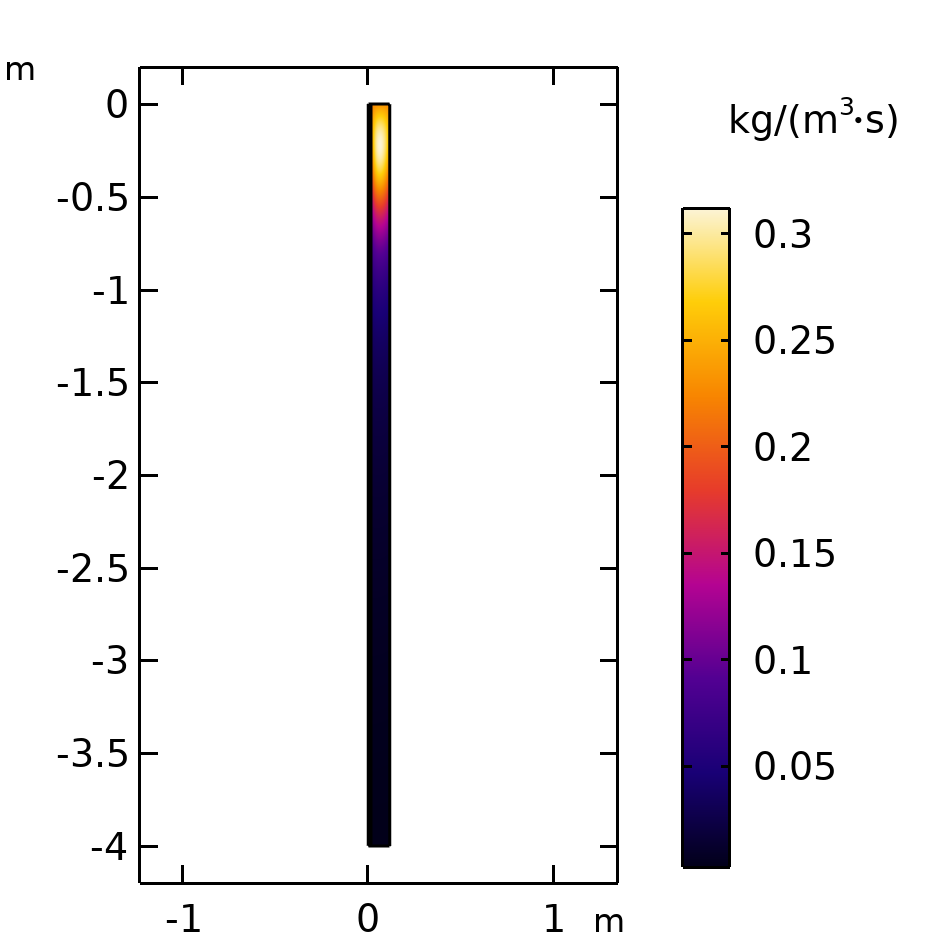
\includegraphics[width=\linewidth, scale=0.5]{figures/r_TOL.png}
        \caption{Rate of Toluene reaction}
        \label{fig:comsol-performance:r_TOL}
    \end{subfigure}\hfill
    \begin{subfigure}{0.45\linewidth}
        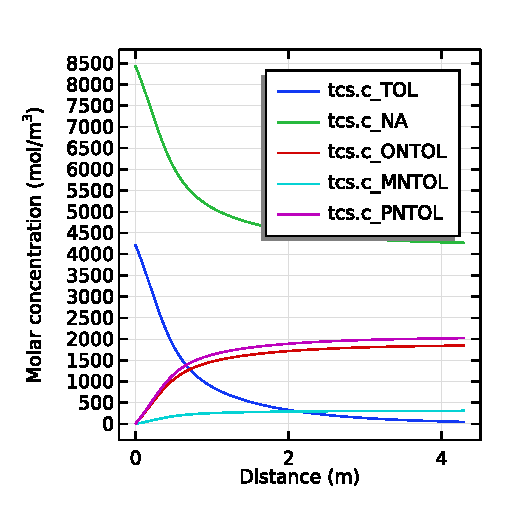
\includegraphics[width=\linewidth, scale=0.5]{figures/concentration.eps}
        \caption{Concentration profile within reactor}
        \label{fig:comsol-performance:concentration}
    \end{subfigure}

    \caption{Reactor performance}
    \label{fig:comsol-performance}
\end{figure}


See \cref{fig:comsol-conversion}.

\begin{figure}[h]
    \centering

    \begin{subfigure}{0.49\linewidth}
        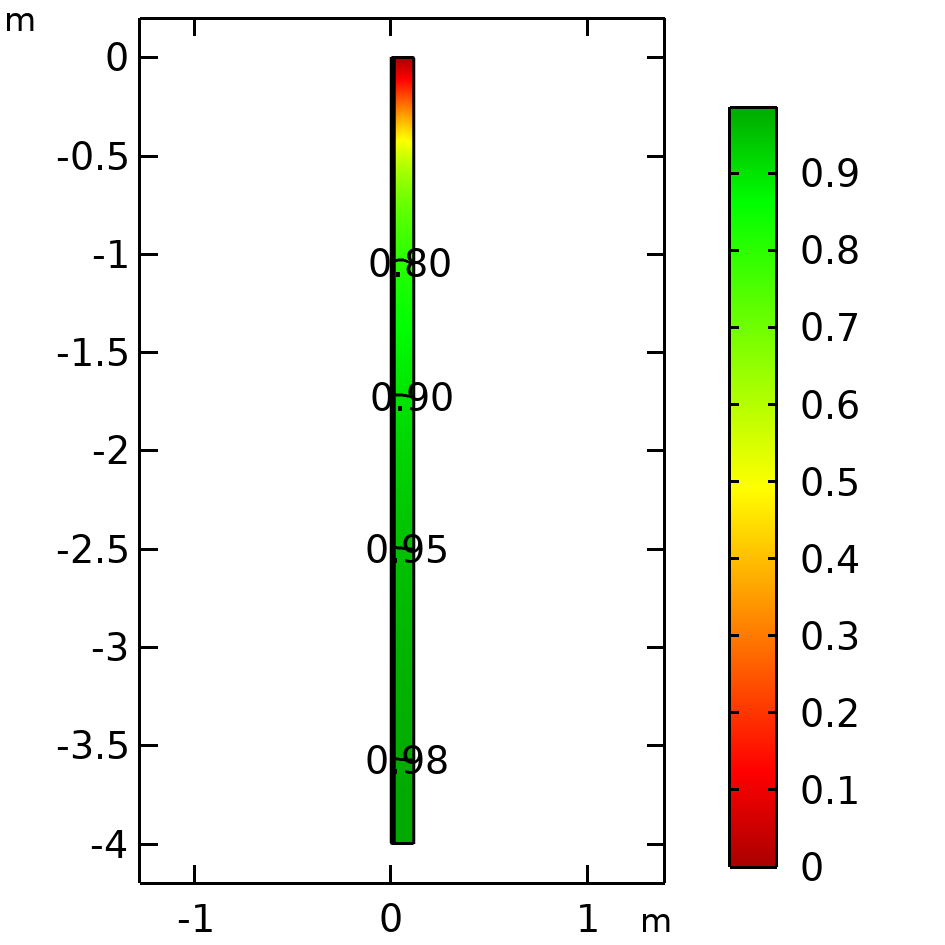
\includegraphics[width=\linewidth, scale=0.5]{figures/conversion-surface.png}
        \label{fig:comsol-conversion:surface}
    \end{subfigure}
    \begin{subfigure}{0.49\linewidth}
        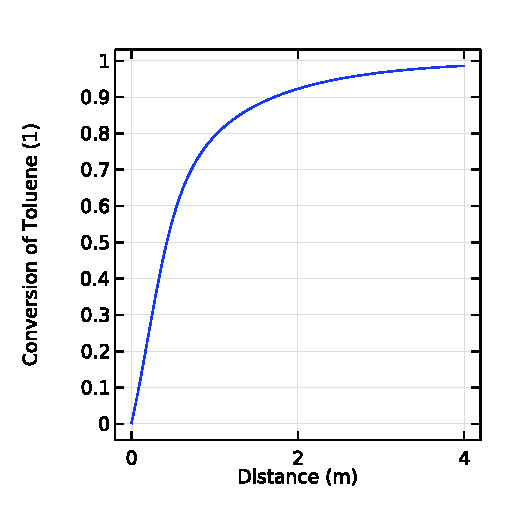
\includegraphics[width=\linewidth, scale=0.5]{figures/conversion-line.eps}
        \label{fig:comsol-conversion:line}
    \end{subfigure}

    \caption{Conversion of toluene across reactor length}
    \label{fig:comsol-conversion}
\end{figure}

The reaction achieves 98\% conversion in 3.6m 

\subsubsection{Temperature}
See \cref{fig:comsol-temperature}.

\begin{figure}[h]
    \centering

    \begin{subfigure}{0.32\linewidth}
        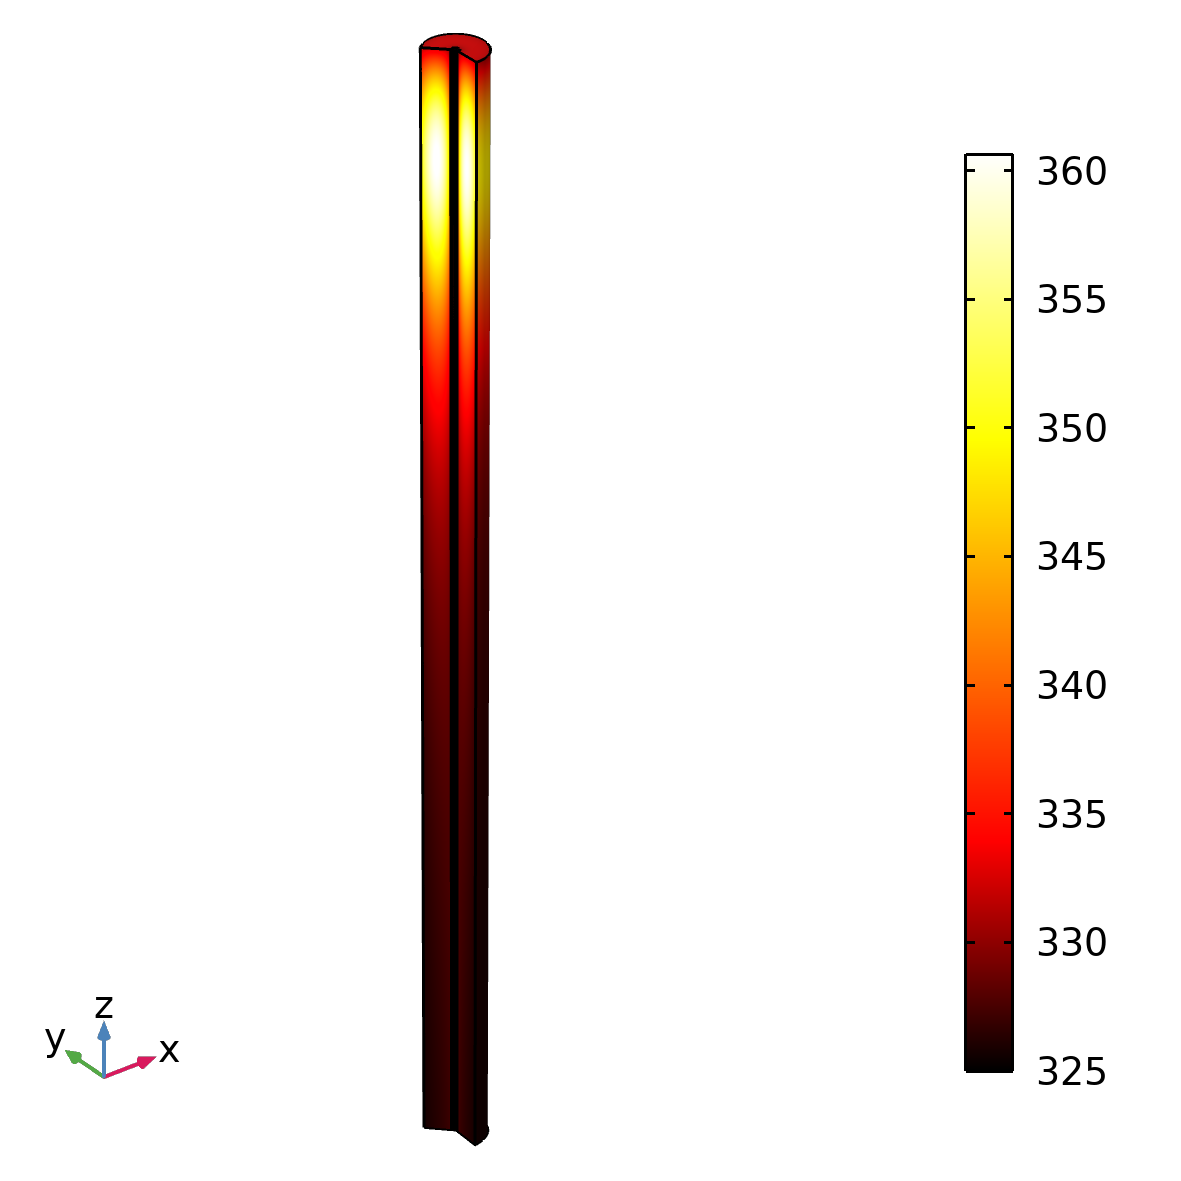
\includegraphics[width=\linewidth]{figures/temperature-surface.png}
        \caption{Overall profile}
        \label{fig:comsol-temperature:surface}
    \end{subfigure}
    \begin{subfigure}{0.32\linewidth}
        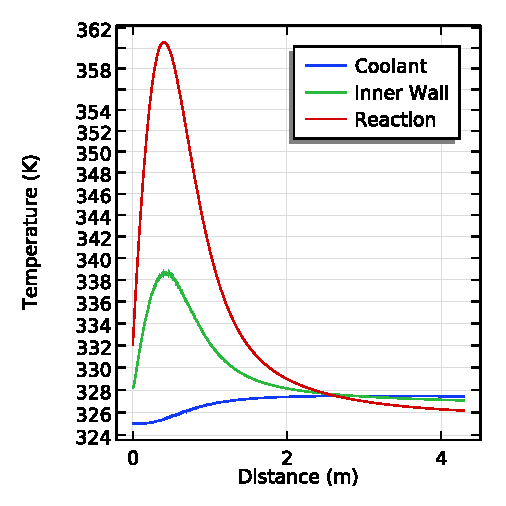
\includegraphics[width=\linewidth]{figures/temperature-lines.eps}
        \caption{$T(z)$ within each section}
        \label{fig:comsol-temperature:lines}
    \end{subfigure}
    \begin{subfigure}{0.32\linewidth}
        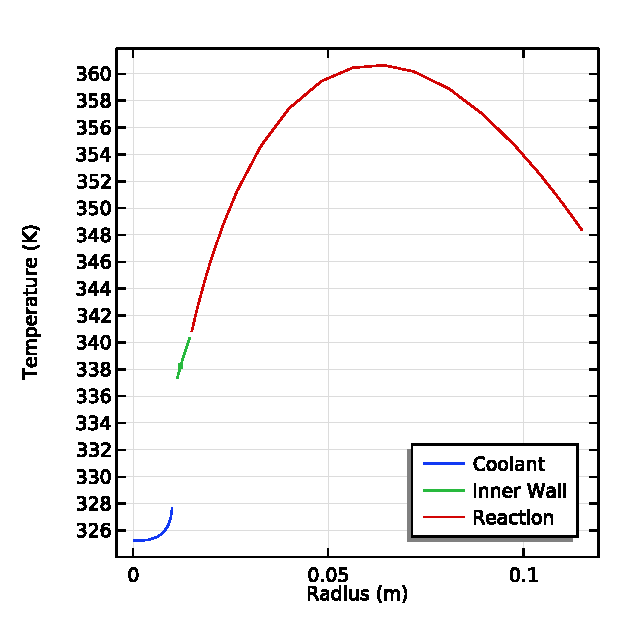
\includegraphics[width=\linewidth]{figures/Tr-maxT.eps}
        \caption{$T(r)$ at $T = \max(T)$}
        \label{fig:comsol-temperature:radial}
    \end{subfigure}

    \caption{Temperatures in reactor}
    \label{fig:comsol-temperature}
\end{figure}